\documentclass{article}
\usepackage[utf8]{inputenc}
\usepackage{graphicx}
\usepackage{float}
\usepackage{enumerate}
\usepackage{parskip}
\usepackage[numbers, sort]{natbib}
\usepackage{hyperref}

\title{Project Initiation Document \\ Conformance checking using activity and trace embeddings}
\author{Group 5 }
\date{December 2020}

\usepackage{natbib}
\usepackage{graphicx}

\begin{document}

\maketitle

\newpage
\tableofcontents
\newpage

\section{Introduction}
In this project, we aim to implement software for conformance checking using activity and trace embedding for the A1 GmbH, which is a consulting company wanting to optimize their service. This initiation document contains every detail for initiating this project.

In chapter 2, the business cases, for which the product will be developed, will be presented. The financial importance of our product for the client will be explained and two scenarios where our product can be used to improve the service provided by the A1 GmbH will be listed.

In chapter 3, to discuss the feasibility of our product, the concepts and tools that will be used to implement our product will be introduced. Two use cases will also be given to show the applicability of our product.

In chapter 4, a GANTT chart outlining the time frame of our project, and its explanation will be provided.

In chapter 5, tools that will be used in this project and the reason why we choose to use these tools will be given.

In the final chapter, an overview of our development team will be provided, which contains information about our background, academic interests, strengths, and weaknesses as well as the roles assigned to each member of our team.

\section{Business Case}
\subsection{Client}
Our client A1 GmbH is a consulting company that offers business solution products to its customers based on process mining. Current products utilize the PM4Py library for process mining. The products are offered in forms of services, which leads to a high scalability of the product line. A1 GmbH is expecting to achieve more diversity in its product family, such that it results in a broad customer spectrum. They are expecting to enrich their process mining products with strong conformance checking features provided by OURPRODUCT. The following paragraphs will provide two exemplary use cases. The examples show that the solutions provided by A1 GmbH to its customers can be clearly improved by applying OURPRODUCT, leading to higher revenue for A1 GmbH.

\subsection{Example 1: Online Shopping Platform}
B1 GmbH is an online shopping platform with many different types of items. Improving customer experiences is critical for achieving more sales, which can be accomplished by avoiding redundant steps during the order process. B1 GmbH is expecting to offer a better customer experience by examining customer behaviors, which start from accessing the shopping platform and end with placing an order or leaving the website. Every action executed by customers will be internally documented. This produces sufficient data not only for applying OURPRODUCT’s advanced process mining techniques but also for applying its robust conformance checking methods. B1 GmbH will be able to adjust their platform according to the obtained overview of customer behavior using OURPRODUCT. B1 GmbH is planning to purchase the service from A1 GmbH since it has shown its adaptability and effectiveness to their business cases. Important criteria of B1 GmbH for applying OURPRODUCT are:
\begin{enumerate}[i.]
\item Improvement of customer experience
\item Higher Conversion Rate
\end{enumerate}

\subsection{Example 2: Analyzing Repair Process}
C1 GmbH is a mobile device manufacturer with diverse product lines such as smartphones, tablet PCs, and Laptops. Besides the quality and the price competitiveness of the products, C1 GmbH is putting effort into improving customer services during the repair process.  This can result in a better reputation for C1 GmbH, which will result in benefits while competing with other manufacturers on the market. They have been using optimized processes for handling customers' requests, and are expecting to achieve more efficiency.  Every step in a repair process will be documented due to customer production law. This will result in a sufficient amount of data, which can be used by OURPRODUCT’s advanced process mining and conformance checking approach. With the help of OURPRODUCT, C1 GmbH will be able to reduce customer complaints during the repair process, by predicting when and why the products can cause defects. The important criteria of C1 GmbH for applying OURPRODUCT is:
\begin{enumerate}[i.]
\item Avoiding redundant steps during the repair process for better customer experience
\item Finding and solving the weaknesses of the current processes of repair services
\end{enumerate}

\subsection{Benefits}
OURPRODUCT can be applied by A1 GmbH in various aspects. A1 GmbH can offer its existing products to its customers in combination with OURPRODUCT to meet the increasing demand and complexity of data analytics in the market. The above two examples also show that the application of OURPRODUCT is not limited to specific areas of the industry. Considering these factors, A1 GmbH will be able to achieve high revenue after exceeding the break-even point, which was set initial investment on the cost of purchasing and adapting OURPRODUCT to its product line. 

\section{Feasibility Study}

\subsection{Theoretical and Technical Feasibility}
The field of process mining is divided into two main research areas - discovery and conformance checking.
Our product will focus on the latter due to the availability of a wide range of tools for the former, e.g. alpha miner \cite{alphaminer} and its improved variants.
Given a model, one wants to assess its quality.
For this, the model is usually compared to real-world process logs.
As these models and logs are in most cases large, automated approaches are necessary.
The already proposed methods can be approximately divided into two groups: log replay based and trace alignment based \cite{thebible}.
To outperform these existing approaches, we want to try a completely new method based on embeddings as proposed in the work by Peeperkorn et al. \cite{source}.
The usage of a novel method immediately raises the question of feasibility.
The main concerns are:
\begin{enumerate}
    \item Is the approach fast enough?
    \item How high is the implementation time?
    \item Does the novel approach deliver good results?
\end{enumerate}

\paragraph{Performance} The performance of an algorithm is a critical factor for the practical employment of the method.
If the time to completion of an algorithm is too high, it might not be feasible to use it in a production setting.
The approach we want to take has already been investigated for performance \cite{source}, showing technical feasibility of the processing of large event logs on a moderate processor.
If higher performance is necessary, this could be achieved by faster machines, performance optimizations of the code (e.g. using a more native programming language like C/C++ or Rust), or the usage of parallelization (e.g. processing multiple parts of the log in parallel).

\paragraph{Implementation} To accelerate the implementation of OURPRODUCT we want two take a two-fold approach:
First, we will utilize the "standing on the shoulders of giants"-principle by using existing well-performing libraries and frameworks like Python, PM4Py \cite{pm4py} and NumPy \cite{numpy}.
Please also refer to the following subsection for further details on these.
Second, we can base our approach on the workflow outlined in the work of Peeperkorn et al. \cite{source}.
For further details regarding our schedule please refer to the GANTT chart provided below.

\paragraph{Quality} The correct behavior of the approach was already verified \cite{source}.
Additionally, one can swap out individual parts of the approach with different algorithms.
Together with the parameter space, this delivers room for improvement of the quality if necessary.

\subsection{Use Cases}

\subsubsection{Python}

Mathematics can be seen as a core discipline present in all kinds of sciences like physics, chemistry and, biology as many problems in those fields are solved using mathematical tools. Therefore, most scientists have a good grasp of how to describe field-specific tasks in the universal language of mathematics. Today, in the age of computers, a new joint-discipline has arisen: powerful computers can be used to tackle complicated tasks that could not be solved before. To do this, however, one needs to know a programming language to reformulate a problem so that a computer can solve it. For many programming languages, this often means that one needs to be able to think like a computer scientist. Because many experts have never dealt with any aspect of computer science, this poses a problem because, now, two people are needed to perform one task - one person with expertise in a given domain and one person with expertise in computer science. 

The programming language Python aims to loosen this dependency by using formulations that look similar to mathematical expressions and by providing libraries for almost any scientific discipline. Examples, among many more, are \textit{Astropy} for astronomy, \textit{Biopython} for biology, \textit{Matplotlib} and \textit{Seaborn} for any kind of data visualization and \textit{Numpy} for efficient computation of all kinds of mathematical calculations.

Summarizing, the benefits of using Python in a scientific environment are:

\begin{itemize}
    \item Simplicity: fast translation of scientific tasks/ problems into the Python programming language without prior knowledge in computer science.
    \item Availability: huge amount of well-documented, domain-specific libraries that are often based on scientific papers.
    \item Versatility: Python can be used for almost anything ranging from pure mathematical calculations to big applications with a graphical user interface.
\end{itemize}

\subsubsection{Conformance Checking}

The Seoul National University Bundang Hospital (SNUBH) is one of the major hospitals in Korea with 1,356 beds and more than 4,500 patients that visit the hospital every day. Such numbers make the healthcare processes very complicated and therefore the hospital would like to see if the processes that patients actually follow still match the standard processes of the hospital. This gets even more interesting, as the standard model of the hospital dates back to a time where there were fewer patients. To find out if the standard model was still up to date, the Ulsan National Institute of Science and Technology (UNIST) applied methods from the field of conformance checking to compare the standard model with the actual processes. \cite{case_study_2014}

\begin{enumerate}
    \item The event log was extracted from the hospital information system and contained:
    \begin{itemize}
        \item About 120,000 cases (treated patients)
        \item About 700,000 events (activities performed for these patients)
        \item 15 different tasks
    \end{itemize}
    \item Together with the medical professionals, the following questions were posed:
    \begin{itemize}
        \item Does the standard model explain actual patients' movements in the hospital?
        \item How much of increase in patients is allowed?
        \item Are the process patterns different depending on the patient types?
    \end{itemize}
    \item The results were as follows:
    \begin{itemize}
        \item It was found that the actual outpatient care processes were much more complex than depicted in the standard model. However, the medical staff explained this with the fact that the standard model only shows the most important flows. Apart from that, the professionals were not able to find any undesired deviations in the derived model which means that the processes are well-managed by the hospital.
        \item An increase of patients of less than 10\% was advised by the data analysts to prevent a big increase in the consultation waiting time for patients
        \item Further analysis found that there were differences in process patterns between new patients and returning patients and that new patients stayed longer than returning patients. The results of the pattern analysis were used to develop a smart healthcare system in the hospital. Patients can now use a smartphone to find their route that is recommended based on the pattern analysis result.
    \end{itemize}
\end{enumerate}

The results show that the overall process model of the hospital is still up to date, even with the increase of patients. Through the pattern analysis, a smart app could be developed to make the patients' journey through the hospital easier and more efficient. Additionally, the medical experts were informed that a large increase in patients might result in much higher consultation waiting times for the patients. The staff of the hospital were impressed by the results and requested further analyses concerning the call center and the payment process models.

\section{Project Charter}
The timeline of our project can be seen in the following GANTT Chart:

\begin{figure}[H]
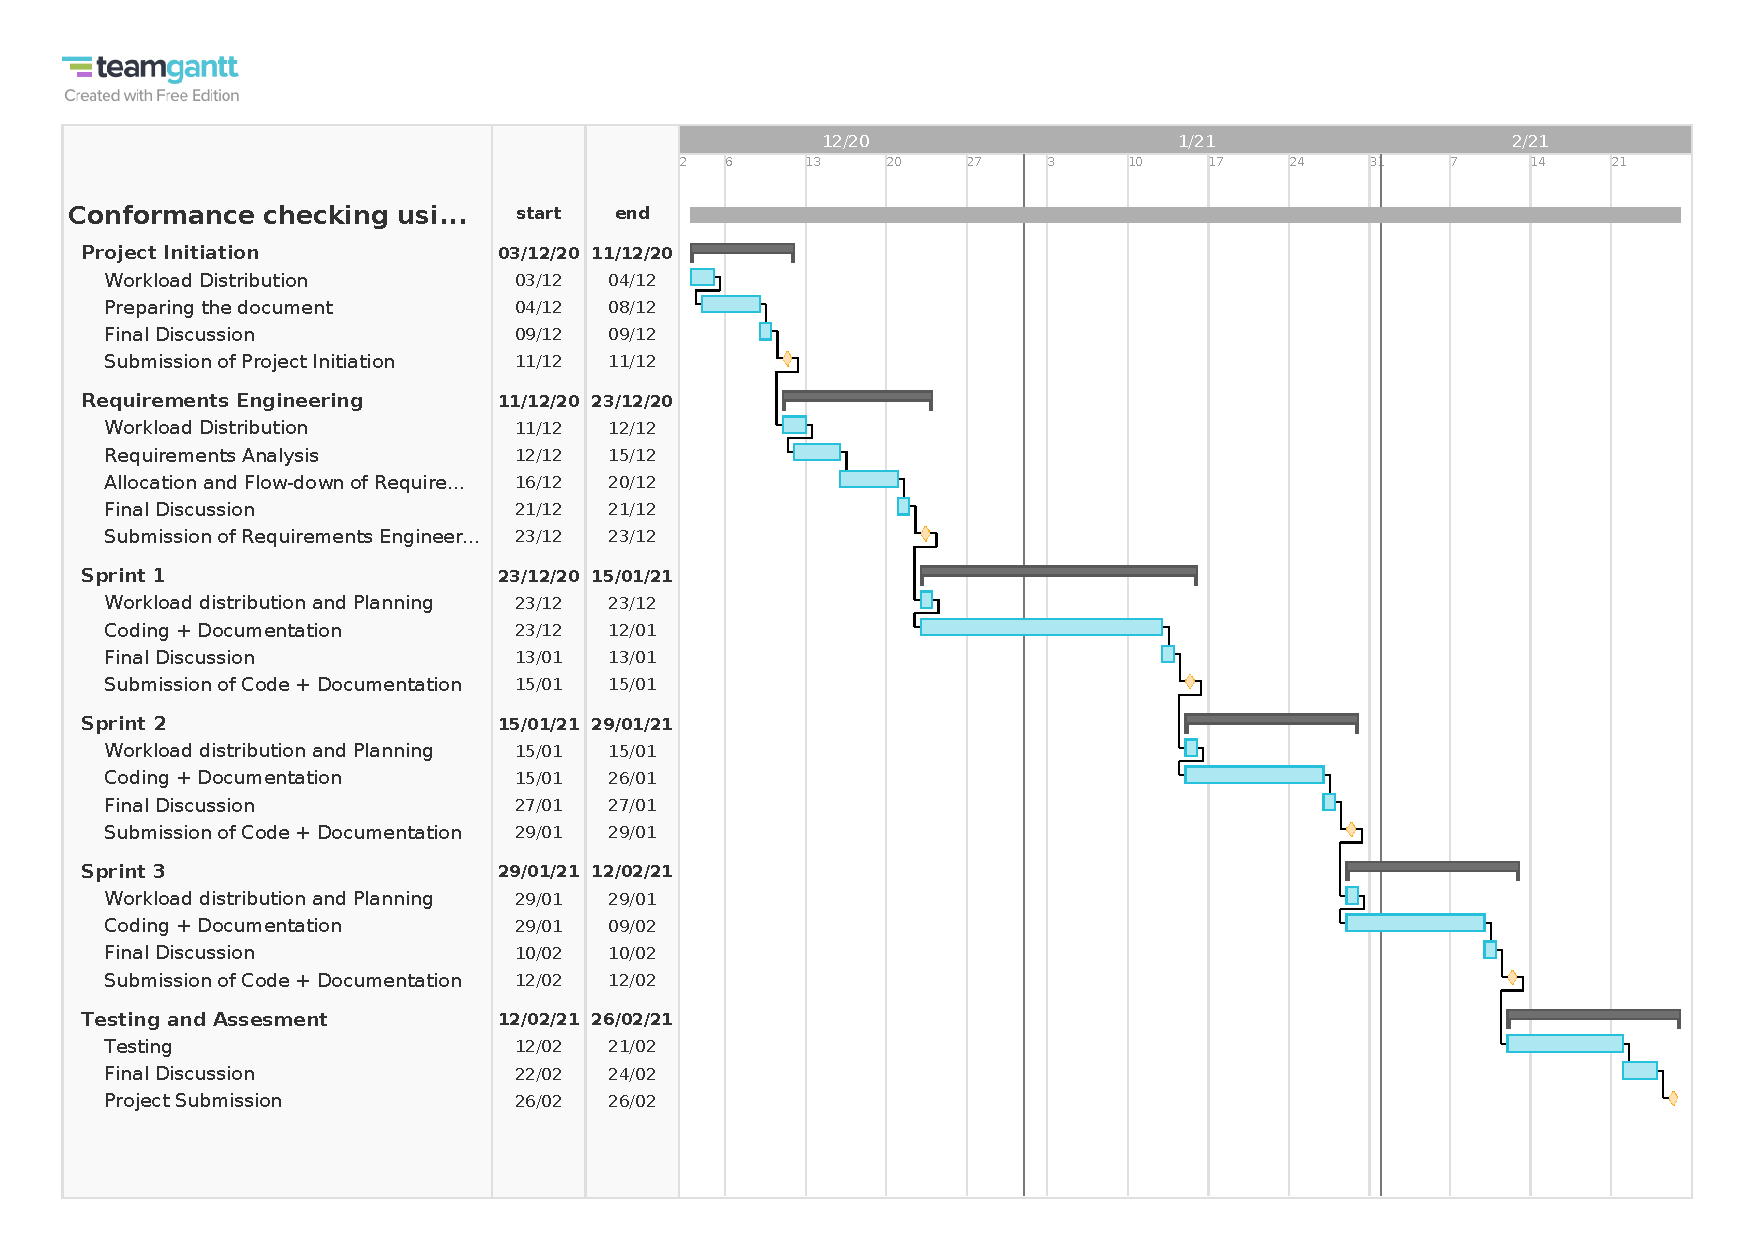
\includegraphics[width = 12cm]{GANTT Chart.pdf}
\end{figure}

Our plan follows a distinct pattern. We always start with a Planning phase, which mostly consists of workload distribution and planning of any internal deadlines. Then every team member has time to accomplish his tasks until the Final Discussion deadline, which is for the most part a couple of days before any given milestone. The deadlines are not set with too much time after them, since we believe that feedback should not only be given at a strict time but at any time, giving the corresponding person enough time to fix any mistakes and not waste any time on things that may ultimately need to be changed completely. These deadlines are nonetheless a few days before the milestones since it is also important to gather our feedback and reflect on what we've accomplished, whilst also having some time for any small changes before the milestone.\\
Our sprints are roughly 2 weeks each, with 11 days for development and documentation, followed by 3 days for discussions and final changes.\\
The main \textbf{Milestones} and their respective dates of our project are the submissions of any work product connected to the following:
\begin{itemize}
    \item Project Initiation: 11 December 2020 (23:59:59 CET)
    \item Requirements Engineering: 23 December 2020 (23:59:59 CET)
    \item Sprint 1: 15 January 2021 (23:59:59 CET)
    \item Sprint 2: 29 January 2021 (23:59:59 CET)
    \item Sprint 3: 12 February 2021 (23:59:59 CET)
    \item Testing and Assessment: 26 February 2021 (23:59:59 CET)
\end{itemize}

It is important to note that this is a preliminary planning of our project, which is subject to change due to the current COVID-19 pandemic, as well as any personal/professional hurdles that may arise during the execution of the project. 

 \section{Tools}
 \subsection{Trello}
 We use Trello, which is a web-based platform to assist, organize, and plan our project. Every member of our group has access to plenty of useful tools that helps with our teamwork and the definition of tasks. In this platform, we can create lists and divide them into smaller tasks, which allows us to assign them to our team members. To enhance our project, we mark the most important tasks with proper color labels and set deadlines. If someone finishes his work, he can check the list and complete the assigned task. Altogether, Trello is a user-friendly platform, that plays a significant part in our project.\\ \\
 Link to our Trello board: \href{https://trello.com/b/UoTtYNXr/conformance-checking-group-5}{Group 5 Trello}
 \subsection{GitLab of the RWTH Aachen University}
 RWTH Aachen is a member university of NFDI4Ing and the students have the admission to use DFN AAI Single Sign-On to create projects and groups. We use GitLab of the RWTH Aachen University to manage our own Git-repository so that each team member has access to our project and to increase the quality of the code. Besides, this website has other functions as an issue-tracking-system, a wiki, and an option to review codes. The advantage of utilizing GitLab is that external users can authenticate via GitHub, however, they do not have the access to create groups and projects.\\ \\
 Link to our repository: \href{https://git.rwth-aachen.de/chan.yong.lee/conformance-checking}{Group 5 GitLab}

\subsection{PM4Py}
To implement conformance checking in Python, we use the library, PM4Py, which supports every tool for process mining algorithms. It is an open-source tool and intended to be used in both academia and industry projects, which is developed by the Fraunhofer Institute for Applied Information Technology. This library provides a simplified interface for conformance checking, which has two important techniques: token-based replay and alignments. Therefore, PM4Py is fundamental to complete our project.
\section{Team}

\subsection{Personal Description}

% Tilman: I would suggest we order the descriptions in alphabetic order.

\subsubsection{Chan Yong Lee}
I am a bachelor computer science student in 5th semester at RWTH Aachen University, with business administration as a secondary subject. I have experiences with solving simple problems using Java, C and Python, and I am currently learning iOS application development. I am very interested in applying theories from computer science to solve practical problems, and that have led me to process mining. My strength lies in applying existing methods and developing them furthermore to solve new problems. But since I lack in practical experiences regarding that capability, I believe that this lab course is an excellent opportunity for me. I am expecting to enhance my Python skills and mainly the knowledges about process mining through working in a group to solve practical issues. Furthermore, I am expecting to study more about this field in upcoming semesters, after earning an initial experience from this course.

\subsubsection{Chenyang Li}
I am a Computer Science student in 5th semester at RWTH Aachen University with Electronics as my secondary subject. I have basic knowledge in C, Python and Java, and tried to solve problems in Embedded Software Development, Data Science and Software Engineering. Because of large interest in Data Mining, I attend many courses about it in this semester, for instance, Machine Learning and Introduction to Data Science, which I think maybe helpful for finishing this project. Process Mining is also an important theme in Data Science, so I decide to attend this course. In this project I hope I can work in a team to complete the given tasks, so that I can learn more about Process Mining and improve my programming skills.

\subsubsection{Denis Razsolkov}
I am a Computer Science Bachelor student at RWTH Aachen University with Medicine as a secondary subject. So far I've dabbled with all sorts of programming languages such as JS, Java, Haskell, C++, C\#, etc. in my programming journey. One of the newest additions to my arsenal is Python. I have mainly used Python in Coding Challenges, which I enjoy doing as a way to keep my mind sharp and adaptive to all sorts of situations, as problem-solving is, in my opinion, the most important quality in programming. I've also taken the course "Intro to scientific programming with Python", which gave me a brief overview of the applications of Python in Data Science. This is the reason I decided to attend this Praktikum. Another great aspect of this project is the ability to earn first-hand experience in project management and teamwork. I tend to focus more on the practical implementations of algorithms, rather than the theory behind them. That said I've gained substantial knowledge of various algorithms throughout my studies. I am really looking forward to seeing this project through.

\subsubsection{Hanbit Chang}
I am studying Computer Science Bachelor at RWTH Aachen University, with Business Administration as a secondary subject. I have gained basic knowledge in Java, C and Python by attending various of courses in the university and have practical experience with program C as working as an academic assistant. After participating the course Database and Information System and Business Process Intelligence, I started to get interested in Data science and look forward discover much more about this field, which includes Process Mining. Furthermore, I applied for this project, to gain knowledge about Process Mining and to improve my programming skills in Python. Therefore, it is a great opportunity for me, participating in this project, to expand my practical experience. Through this course, I expect to work together with our group as a team to accomplish the given tasks and successfully complete our project.

\subsubsection{Robin Schmitt}
I am currently pursuing my Bachelor's degree in computer science at the RWTH Aachen University with psychology as an application subject. I was always stunned by the fact that computers seemed to be able to attain human intelligence and beat them, for example, in games that they, themselves invented. This led me to the field of machine learning and subsequently to the broader field of data science which demystified the so-called artificial intelligence for me. Currently, I possess a lot of theoretical knowledge about various machine learning and data science algorithms and I now aim to learn more about the practical applications of those methods, which is why I chose the subject of process mining. I am looking forward to working together with my team members and I hope to be able to contribute to a successful outcome of our project by using my theoretical knowledge and my Python programming skills.

\subsubsection{Tilman Hoffbauer}
I started coding in secondary school for my "Jugend forscht" projects. I am thus an experienced programmer looking into expanding his theoretical knowledge by the study of computer science at the RWTH Aachen University aiming for a B. Sc. at the end of next semester. My main interest lies in the applications of computer science in other domains to accelerate research and innovation. This often includes the application of data science. Process mining is an interesting sub-field of data science showing some very useful applications which easily give high benefit to process managers \& engineers. During the lab, I want to get hands-on experience with process mining after taking a theoretical introductory course by Prof. Wil van der Aalst.

\subsection{Roles}
\paragraph{Scrum Master: Hanbit Chang}
As a scrum master, he is responsible for the organizational environments of his team to create a high-value product. He must manage the Trello Board and GitLab of the project, assign tasks to each member and help the team to approach their work without difficulty.

\paragraph{Official Communication/Product Owner: Chan Yong Lee}
He is responsible for establishing a communication channel between our group and teaching assistants. He will be arranging meetings, delivering tasks and requests so that the project can achieve its goal in an optimal way.

\paragraph{Tools Administration: Denis Razsolkov} As a tools administrator, he should have a good understanding of the tools we might need during the project and be able to introduce everyone on the team to them to assure seamless integration of the tools in our workflow.

\paragraph{Theory Expert: Robin Schmitt} As our theory expert, Robin needs to know the used algorithms and their theoretical background in detail and he should be able to answer any questions that other team members might have concerning the underlying scientific paper.

\paragraph{Software Expert: Chenyang Li}
Working as a software expert, he should be the team member who is very familiar with Python, PM4Py and other libraries that we will use.

\paragraph{Test Management: Tilman Hoffbauer}
As the test manager, he is responsible for the organization and orchestration of tests.

\section{Phase review}

\subsection{Chan Yong Lee}
"I am very satisfied with the overall procedure that our team has taken to finish our first task in this project. Even though everything should have been done online due to COVID-19 Pandemic, every team member was responsible and finished their assignments. In case of conflicts, we tried to listen to each other's preferences and find the best solution which could satisfy both. Now that every team member has found their positions in this project, and they got used to cooperation tools like Trello and Slack, I am expecting more efficient teamwork in upcoming phases of this project"

\subsection{Chenyang Li}
"This is the first phase of our project. I was scared that lack of communication might cause serious problems at the beginning, but now I would say that we finished it somehow perfectly. All communication seemed to flow well, and members were very active in giving their opinions. We held a short meeting at first to divide this long document into many short pieces, then we only focused on our own part and took a review to the other parts, this made us work efficiently. Overall, the first phase is a good starting phase for all of us, so I am confident that we can finish this project perfectly."

\subsection{Denis Razsolkov}
"I entered this project being somewhat unsure of how well we will be able to work together as a team. Due to the current COVID-19 events I expected some problems with our planning and overall communication. All my worries proved to be unfounded. I am happy to say that ever since our first meeting we were able to accomplish our tasks swiftly without compromising the quality of our work. Our communication and planning also went smoothly thanks to the tools we used to implement in our workflow. Overall I think this first phase of our project was a great success and I am really looking forward to working together and seeing this project through."

\subsection{Hanbit Chang}
“I am very excited to have my first practical experience participating in a software project with my great team. Due to current situation of COVID-19 Pandemic, it was not possible for us to have our first meeting in person, however we managed to organize and plan through our project. Our teamwork went fluently by utilizing platform as Trello to assign tasks for each member and check the finished tasks. We communicated through Slack and kept on giving feedbacks to each other. Thankfully, we were always ready to quickly response and improve the quality of our project. We finished our first assignments and expect us to complete the upcoming phases of this project without difficulties”

\subsection{Robin Schmitt}
"This is the first software project where I am working together with a team. The most exciting part for me was, that we all did not know each other beforehand and therefore I was not sure if the project coordination would work out. Surprisingly, our first online meeting was very productive and we were able to assign tasks to every group member and that without any conflicts. This was different to other group assignments I did in the past, where I mostly knew my fellow group members and we therefore often ended up talking more about leisure than about the actual work. Because of this, I am confident that the following weeks are going to be productive and I am looking forward to continue working on our project."

\subsection{Tilman Hoffbauer}
"First, I was unsure whether we would manage to organize us as a team due to the reduced communication implied by the COVID-19 pandemic.
But we did a good job without a personal meeting.
With the help of the various online tools, we could work very efficiently - maybe even more efficient than with a regular in-person group meeting.
For the situations, where a personal discussion was more appropriate, we concluded two Zoom meetings.
We established some good communication protocols and formed a well-organized team, so I expect productive teamwork in the next weeks!"


\bibliographystyle{plain}
\bibliography{references}
\end{document}
